\documentclass[12pt]{article}
\usepackage[width=16cm]{geometry}                % See geometry.pdf to learn the layout options. There are lots.
\geometry{a4paper}                   % ... or a4paper or a5paper or ... 
%\geometry{landscape}                % Activate for for rotated page geometry
%\usepackage[parfill]{parskip}    % Activate to begin paragraphs with an empty line rather than an indent
\usepackage{graphicx}
\usepackage{amssymb}
\usepackage{amsmath}
\usepackage{aliases}
\usepackage{color}
\usepackage{url}

\usepackage{listings}
\usepackage{cancel}
\usepackage{textcomp}

\lstset{
   language=matlab,
   keywordstyle=\bfseries\ttfamily\color[rgb]{0,0,1},
   identifierstyle=\ttfamily,
   commentstyle=\color[rgb]{0.133,0.545,0.133},
   stringstyle=\ttfamily\color[rgb]{0.627,0.126,0.941},
   showstringspaces=false,
   basicstyle=\small,
   numberstyle=\footnotesize,
   numbers=none,
   stepnumber=1,
   numbersep=10pt,
   tabsize=2,
   breaklines=true,
   prebreak = \raisebox{0ex}[0ex][0ex]{\ensuremath{\hookleftarrow}},
   breakatwhitespace=false,
   aboveskip={0.1\baselineskip},
    columns=fixed,
    upquote=true,
    extendedchars=true,
% frame=single,
    backgroundcolor=\color[rgb]{0.9,0.9,0.9}
}

\title{Linear control of inverted pendulum}
\author{Deep Ray, Ritesh Kumar, Praveen. C, Mythily Ramaswamy, J.-P. Raymond}
\date{}

\begin{document}



\maketitle

\begin{center}
IFCAM Summer School on Numerics and Control of PDE\\
22 July - 2 August 2013\\
IISc, Bangalore\\
\url{http://praveen.cfdlab.net/teaching/control2013}
\end{center}


\section{Inverted pendulum}
\begin{center}
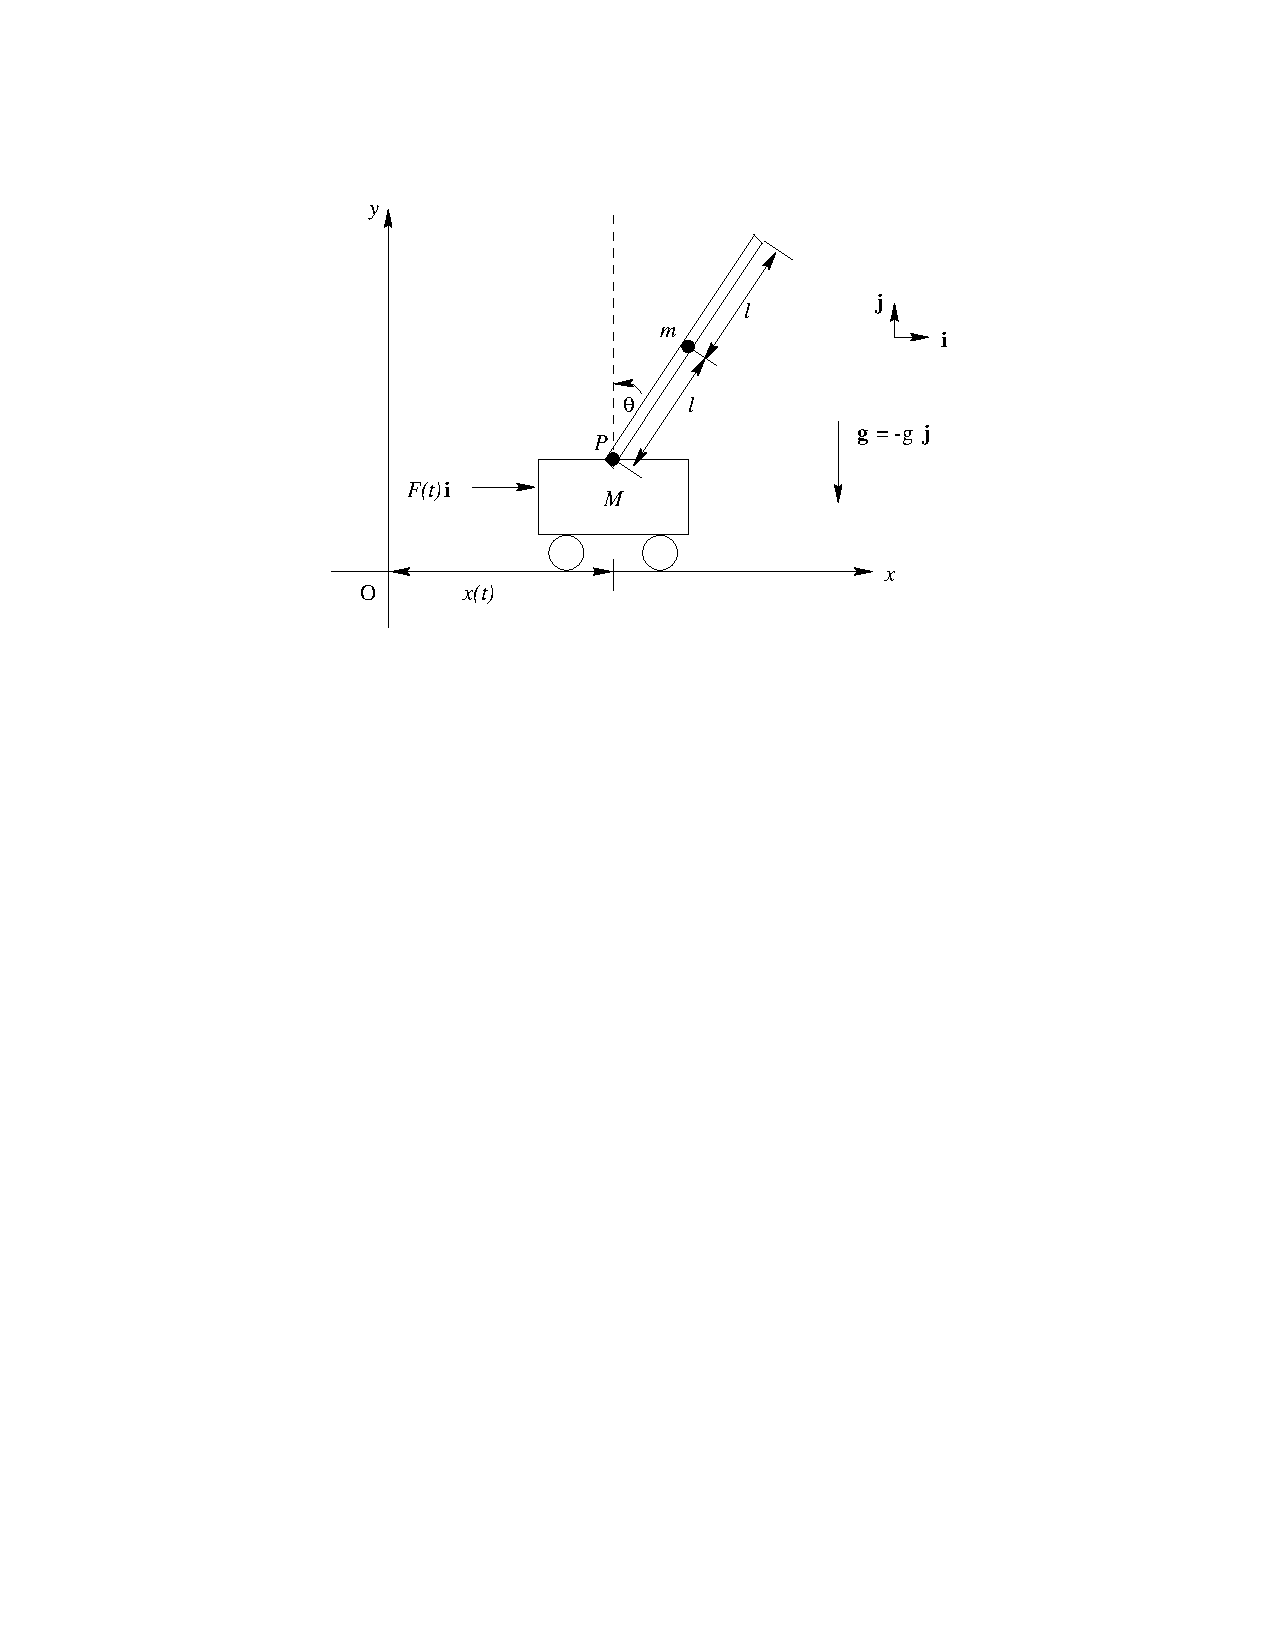
\includegraphics[width=0.50\textwidth]{inv_pendulum}
\end{center}
\[
I = \mbox{Moment of inertia of pendulum about its cg} = \frac{1}{3} m l^2
\]
Lagrangian
\[
L = \frac{1}{2} M \dx^2 + \frac{1}{2}m(\dx + l \dt \cos\theta)^2 + \frac{1}{2}(I+ml^2)     \dt^2 - mgl\cos\theta
\]
Euler-Lagrange equation
\[
\dd{}{t} \left(\df{L}{\dx}\right) - \df{L}{x} = F, \qquad \dd{}{t} \left( \df{L}{\dt}      \right) - \df{L}{\theta} = 0
\]
gives
\begin{eqnarray*}
(M+m) \ddx + m l \ddt \cos\theta - m l \dt^2 \sin\theta + k \dx &=&  F \\
m l \ddx \cos\theta + (I+ml^2) \ddt - mg l \sin\theta + c \dt &=& 0
\end{eqnarray*}
This is a coupled system
\[
\begin{bmatrix}
M+m & m l \cos\theta \\
m l \cos\theta & I + ml^2 \end{bmatrix}
\begin{bmatrix}
\ddx \\ \ddt \end{bmatrix} = \begin{bmatrix}
m l \dt^2 \sin\theta - k \dx + F \\
mg l \sin\theta - c \dt \end{bmatrix}
\]
Define determinant
\[
D = (M+m)(I+ml^2) - m^2 l^2 \cos^2\theta
\]
Solving for $\ddx$, $\ddt$
\[
\begin{bmatrix}
\ddx \\ \ddt \end{bmatrix} = \frac{1}{D} \begin{bmatrix}
m l \cos\theta (c \dt - mgl\sin\theta) + (I+ml^2)(F - k\dx + ml\dt^2 \sin\theta) \\
(M+m)(-c\dt + mgl\sin\theta) - ml\cos\theta(F - k\dx + ml\dt^2 \sin\theta)
\end{bmatrix}
\]
Define
\[
z = (z_1, z_2, z_3, z_4)^\top = (x, \dx, \theta, \dt)^\top
\]
Then
\[
\dot{z}_1 = z_2, \qquad \dot{z}_3 = z_4
\]
we can write the first order system
\[
\begin{bmatrix}
\dz_1 \\ \dz_2 \\ \dz_3 \\ \dz_4 \end{bmatrix} = \begin{bmatrix}
z_2 \\
\frac{1}{D} [ m l \cos z_3 (c z_4 - mgl\sin z_3) + (I+ml^2)(F - k z_2 + ml z_4^2 \sin      z_3)] \\
z_4 \\
\frac{1}{D}[ (M+m)(-c z_4 + mgl\sin z_3) - ml\cos z_3 (F - k z_2 + ml z_4^2 \sin z_3)]
\end{bmatrix}
\]
In the experimental setup of Landry, the force $F$ on the cart is
\[
F(t) = \alpha u(t) - \beta \dx, \qquad \alpha > 0, \qquad \beta > 0
\]
where $u$ is the voltage in the motor driving the cart, and the second term represents the electrical resistance in the motor. Let us write the non-linear pendulum model as
\[
\dd{z}{t} = N(z,u)
\]
The numerical solution of this model is implemented in program {\tt nlp.m}
%--------------------------------------------------------------------------------
\paragraph{Excercises}
The matlab programs are in the directory {\tt pendulum}; go into this directory and start matlab. E.g. if you are working on the Unix/Linux command line
\begin{lstlisting}
$ cd control2013/pendulum
$ matlab
\end{lstlisting}
If you have started matlab through some other way, then change the directory inside matlab
\begin{lstlisting}
>> cd <Full path to>/control2013/pendulum
\end{lstlisting}
Or use the matlab gui to change the working directory.

The pendulum has two equilibrium positions, one upright ($\theta=0$) and another in the down position ($\theta=\pi$).
\begin{enumerate}
\item Solve the non-linear pendulum problem with initial condition close to upright position 
\[
z(0) = \begin{bmatrix} 0, 0, \frac{5\pi}{180}, 0 \end{bmatrix}
\]
and final time $T=100$. Is the upright position stable ? What happens to the four variables ? Interpret the solution in physical terms.

\item Solve the non-linear pendulum problem with initial condition close to downward position
\[
z(0) = \begin{bmatrix} 0, 0, \frac{170\pi}{180}, 0 \end{bmatrix}
\]
and final time $T=100$. Is the downward position stable ?

\end{enumerate}
%--------------------------------------------------------------------------------
\subsection{Linearised system} 
We linearize around $z=(0,0,0,0)$
\[
\dd{}{t} \begin{bmatrix}
z_1 \\ z_2 \\ z_3 \\ z_4 \end{bmatrix} = \begin{bmatrix}
0 & 1 & 0 & 0 \\
0 & - (k+\beta) v_2 & - \frac{m^2 l^2 g v_2}{I + ml^2} & \frac{ml c v_2}{I + ml^2} \\
0 & 0 & 0 & 1 \\
0 & \frac{ml(k+\beta)v_2}{M+m} & mlgv_1 & - c  v_1
\end{bmatrix} \begin{bmatrix}
z_1 \\ z_2 \\ z_3 \\ z_4 \end{bmatrix} +
\begin{bmatrix}
0 \\ \alpha v_2 \\ 0 \\ -\frac{\alpha mlv_1}{M+m} \end{bmatrix} u
\]
where
\[
v_1 = \frac{M + m}{I(M+m) + mMl^2}, \qquad v_2 = \frac{I + ml^2}{I(M+m) + mMl^2}
\]
then we have the linear model
\[
\dd{z}{t} = Az + Bu
\]
%--------------------------------------------------------------------------------
\paragraph{Excercises}

\begin{enumerate}

\item Generate matrices for linear system
\begin{lstlisting}
parameters
[A,B] = get_system_matrices()
\end{lstlisting}

\item Compute eigenvalues
\begin{lstlisting}
e = eig(A)
plot(real(e), imag(e), 'o')
\end{lstlisting}
Is there an unstable eigenvalue ? Is there a zero eigenvalue ?

\item Check that $(A,B)$ is controllable by computing rank of controllability matrix
\[
P_c = \begin{bmatrix} 
B & A B & A^2 B & A^3 B
\end{bmatrix}
\]
\begin{lstlisting}
Pc = [B, A*B, A^2*B, A^3*B];
rank(Pc)
\end{lstlisting}

\item Check the controllability using Hautus criterion. For each eigenvalue $\lambda$, compute eigenvector $V$ of $A^\top$
\[
A^\top V = \lambda V
\]
and check if 
\[
B^\top V \ne 0
\]
If the above condition is true for each unstable eigenvalue, i.e., with $\mbox{real}(\lambda) > 0$, then the system is stabilizable.

\item Solve linear model ({\tt lp.m}) with initial condition 
\[
z(0) = \begin{bmatrix} 0, 0, \frac{5\pi}{180}, 0 \end{bmatrix}
\]
upto a final time of $T=5$. Compare this solution with solution of non-linear model.

\end{enumerate}
%--------------------------------------------------------------------------------
\section{Minimal norm feedback control}
The minimal norm control is given by
\[
u(t) = - K z (t) \qquad\mbox{with}\qquad K = B^\top X
\]
where $X$ is the maximal solution of Algebraic Bernoulli Equation (ABE)
\[
A^\top X + X A - X B B^\top X = 0
\]
For inverted pendulum, matrix $A$ has a zero eigenvalue. We replace $A$ with $A+\omega I$, $\omega > 0$, for determining the control.
\[
(A+\omega I)^\top X + X (A+\omega I) - X B B^\top X = 0, \qquad K = B^\top X
\]
Model with feedback
\[
\dd{z}{t} = (A - BK)z, \qquad z(0) = z_0
\]
%--------------------------------------------------------------------------------
\paragraph{Excercises}

\begin{enumerate}

\item Compute the minimal norm feedback matrix $K$ using {\tt lqr} function
\begin{lstlisting}
Q = zeros(4,4);
R = 1;
om = 0.01;
A = A + om*eye(4);
[K,S,E] = lqr(A, B, Q, R);
plot(real(E), imag(E), 'o')
\end{lstlisting}
$E$ contains the eigenvalues of $A - B K$.

\item Also check for yourself that $A-BK$ is stable by computing its eigenvalues.
\begin{lstlisting}
e = eig(A-B*K);
plot(real(e), imag(e), 'o')
\end{lstlisting}

\end{enumerate}

%--------------------------------------------------------------------------------

\section{Feedback control using LQR approach}
Measurement
\[
y_m = C z, \qquad \textrm{e.g.} \qquad C = I_4
\]
Performance measure
\begin{eqnarray*}
J &=& \frac{1}{2}\int_0^\infty y_m^\top Q_m y_m \ud t + \frac{1}{2} \int_0^\infty u^\top R 
u \ud t \\
&=& \frac{1}{2}\int_0^\infty z^\top Q z \ud t + \frac{1}{2} \int_0^\infty u^\top R u \ud   
t , \qquad Q = C^\top Q_m C
\end{eqnarray*}
Find feedback law
\[
u = -K z
\]
which minimizes $J$. The feedback or gain matrix $K$ is given by
\[
K = R^{-1} B^\top X
\]
where $X$ is solution of algebraic Riccati equation (ARE)
\[
A^\top X + X A - X B R^{-1} B^\top X + Q = 0
\]
%The solution exists if $(A,B)$ is controllable and $(A,C)$ is observable.
%--------------------------------------------------------------------------------

\paragraph{Excercises}

\begin{enumerate}

\item We may observe different quantities, e.g.,
\[
C = \begin{bmatrix}
1 & 0 & 0 & 0 
\end{bmatrix}, \qquad C = \begin{bmatrix}
0 & 0 & 1 & 0
\end{bmatrix}, \qquad C = \begin{bmatrix}
1 & 0 & 0 & 0 \\
0 & 0 & 1 & 0
\end{bmatrix}, \qquad C = \begin{bmatrix}
1 & 0 & 0 & 0 \\
0 & 1 & 0 & 0 \\
0 & 0 & 1 & 0 \\
0 & 0 & 0 & 1
\end{bmatrix}
\]
In each case, check if $(A,C)$ is observable by computing rank of observability matrix
\[
P_o = \begin{bmatrix}
C \\
CA \\
CA^2 \\
CA^3
\end{bmatrix}
\]

\item Compute feedback operator $K$ using {\tt lqr} function. We will control position and angle.
\begin{lstlisting}
C = [1 0 0 0; 0 0 1 0];
Q = C'*C;
R = 1;
[K,S,E] = lqr(A, B, Q, R);
plot(real(E), imag(E), 'o')
\end{lstlisting}
$E$ contains the eigenvalues of $A - B K$.

\item Solve with LQR feedback control. This is implemented in program {\tt pend\_lqr.m} which solves both linear and nonlinear model. Compare the linear and non-linear solutions. Try with $R=0.01$ and $R=0.1$ and initial condition
\[
z(0) = \begin{bmatrix}
0 & 0 & \frac{50 \pi}{180} & 0 
\end{bmatrix}
\]
Which is better ?

\item Run the program {\tt pend\_lqr.m} with different initial angles
\[
z(0) = \begin{bmatrix}
0 & 0 & \frac{50 \pi}{180} & 0 
\end{bmatrix}, \qquad z(0) = \begin{bmatrix}
0 & 0 & \frac{58 \pi}{180} & 0 
\end{bmatrix}
\]
and for $R=0.01$ and $R=0.1$. Which value of $R$ gives faster stabilization ? What is the maximum magnitude of control in each case ? 

\item Find angle beyond which non-linear model cannot be stabilized. Do this for $R=0.01$, $R=0.1$ and $R=0.5$. Use final time of $T=3$ and initial conditions of the form 
\[
z(0) = \begin{bmatrix}
0 & 0 & \theta_0 & 0 
\end{bmatrix}
\]
Use the evolution of energy as an indicator for finding the threshold angle.

\end{enumerate}

%--------------------------------------------------------------------------------

\section{Linear system with noise and partial information}
Consider the system with noise in the model and initial condition
\[
\dd{z}{t} = Az + Bu + w, \qquad z(0) = z_0 + \eta
\]
where $w$ and $\eta$ are error/noise terms. We may not have access to the full state but only some partial information which is also corrupted by noise.
\[
y_o = Hz  + v, \qquad \textrm{e.g.} \qquad H = \begin{bmatrix}
1 & 0 & 0 & 0 \\
0 & 0 & 1 & 0 \end{bmatrix}
\]
which corresponds to observing $x$ and $\theta$.

\vspace{5mm}

Since we have partial information, we estimate $z$ by a linear estimator.
%--------------------------------------------------------------------------------

\subsection{Estimation problem}
Linear estimator
\[
\dd{z_e}{t} = A z_e + Bu + L(y_o - H z_e)
\]
We determine the filtering gain $L$ by minimizing
\[
J = \frac{1}{2} \int_0^\infty (y_o - H z_e)^\top R_v^{-1} (y_o - H z_e) \ud t +            \frac{1}{2} \int_0^\infty w^\top R_w^{-1} w \ud t
\]
The solution is given by
\[
L = - X_e H^\top R_v^{-1}
\]
where $X_e$ is solution of
\[
A X_e + X_e A^\top - X_e H^\top R_v^{-1}  H X_e + R_w = 0
\]

\paragraph{Excercises}

\begin{enumerate}

\item Compute the filtering matrix $L$
\begin{lstlisting}
Rw = (5e-3) *diag([0.9,0.8,0.4,0.7]);
Rv = (5e-3) *diag([0.9,0.8]);
[L, S] = lqr(A', H', Rw, Rv);
L = real(L');
\end{lstlisting}

\item Compute eigenvalues of $A-LH$ and check that they are all stable.

\end{enumerate}
%--------------------------------------------------------------------------------

\subsection{Coupled linear system}
The feedback is based on estimated solution $u = -K z_e$
\begin{eqnarray*}
\dd{z}{t} &=& A z - B K z_e + w \\
\dd{z_e}{t} &=& L H z + (A - B K - L H) z_e + L v
\end{eqnarray*}
or in matrix form
\[
\dd{}{t} \begin{bmatrix}
z \\
z_e \end{bmatrix} = \begin{bmatrix}
A & -B K \\
L H & A - B K - L H \end{bmatrix} \begin{bmatrix}
z \\ z_e \end{bmatrix} + \begin{bmatrix}
I & 0 \\
0 & L \end{bmatrix} \begin{bmatrix}
w \\ v \end{bmatrix}
\]
The initial condition is given by
\[
z(0) = z_0 + \eta, \qquad z_e(0) = z_0
\]
This is implemented in program {\tt lp\_est.m}

\paragraph{Excercises}

\begin{enumerate}

\item Run program {\tt lp\_est.m}

\item The above problem can also be solved without estimation, where the control is generated by the faulty partial observations. For instance, if we observe only the position of the cart and the angle, then the other states can be approximated using a backward time difference. This is implemented in {\tt lp\_noest.m}. Run this code with the same initial conditions and error parameters as chosen in {\tt lp\_est.m}. Which method gives a better control?  

\item Vary the magnitude of the errors (GIVE SOME CHOICES) in the covariance matrices {\tt Rw, Ru}. How does each type of control perform?
\end{enumerate}

%--------------------------------------------------------------------------------

\subsection{Coupled non-linear system}

The feedback is based on estimated solution $u = -K z_e$
\begin{eqnarray*}
\dd{z}{t} &=& N(z, u) + w \\
\dd{z_e}{t} &=& A z_e + B u + L(y_o - H z_e) \\
y_o &=& H z + v
\end{eqnarray*}
with initial condition
\[
z(0) = z_0 + \eta, \qquad z_e(0) = z_0
\]

This is implemented in program {\tt nlp\_est.m}

\paragraph{Excercises}

\begin{enumerate}

\item Run program {\tt nlp\_est.m}

\item Have the threshold angles evaluated for $Ru=0.01$, $Ru=0.1$ and $Ru=0.5$ changed? If yes, then what are the new threshold angles?

\item How does the control vary as {\tt Ru} is changed? Is the behaviour the same as that observed in the earlier cases?

\item How does the value of {\tt Ru} influence the stabilization of the state variables?

\end{enumerate}

%--------------------------------------------------------------------------------

\section{Inverted pendulum: Parameters}

\begin{center}
\begin{tabular}{|c|l|c|}
\hline
$M$ & Mass of cart &  2.4  \\
\hline
$m$ & Mass of pendulum &  0.23 \\
\hline
$l$ & Length of pendulum & 0.36 \\
\hline
$k$ & Friction in cart & 0.05 \\
\hline
$c$ & Friction in pendulum & 0.005 \\
\hline
$\alpha$ & Coefficient of voltage & 1.7189 \\
\hline
$\beta$ &  Friction in motor &  7.682 \\
\hline
$a$ & Acceleration due to gravity & 9.81 \\
\hline
\end{tabular}
\end{center}
%--------------------------------------------------------------------------------

\section{List of Programs}

\begin{enumerate}

\item {\tt parameters.m}: Set parameters for pendulum

\item {\tt get\_system\_matrices.m}: Computes matrices for linear model

\item {\tt hautus.m}: Checks the stabilizability of the system using Hautus criterion
\item {\tt rhs\_nlpc.m}: Computes right hand side of non-linear model, with feedback
\item {\tt rhs\_lp.m}: Computes right hand side of linear model, without feedback

\item {\tt rhs\_nlp.m}: Computes right hand side of non-linear model, without feedback

\item {\tt rhs\_lpc.m}: Computes right hand side of linear model, with feedback

\item {\tt rhs\_nlpc.m}: Computes right hand side of non-linear model, with feedback

\item {\tt rhs\_nlpest.m}: Computes right hand side of non-linear model coupled with the linear estimator and feedback

\item {\tt lp.m}: Solves the linear model without feedback

\item {\tt nlp.m}: Solves the linear model without feedback

\item {\tt pend\_lqr.m}: Solves the linear and non-linear models with feedback and full state information

\item {\tt lp\_est.m}: Solves the linear model with noise and partial information, coupled estimator and feedback stabilization

\item {\tt lp\_noest.m}: Solves the linear model with noise and partial information, feedback without estimation

\item {\tt nlp\_est.m}: Solves the non-linear model with noise and partial information, coupled estimator and feedback stabilization

\end{enumerate}

\end{document}  